\chapter{Methods}\label{chap:2}

Before starting to build a model that is able to predict whether a proposal is going to be accepted or not, it is necessary to explore the dataset to better understand the structure of the data, and gain the first insights. Afterwards, predictive modeling will be carried out and the particularities of the models developed will be discussed. Lastly, the predicted outcomes will be assessed to draw conclusions. 

We begin by analyzing the numerical features in subsection \ref{sec:numfeat}. Then we continue by evaluating the categorical features on subsection \ref{sec:catfeat}.  
%Once we have the full diagnostic of our data we move onto the section
After this preliminary analysis, we detail in section \ref{sec:build} how we built the model and explained in detail each of the challenges we faced in subsections \ref{sec:skewed} and \ref{sec:corr}. Lastly we have an overview of the evaluation methods used in the classifier in the last subsection \ref{sec:eval}.

The dataset we will work with was obtained after gathering the data generated by citizens in the city of Barcelona that participated actively on the platform during a period of approximately three months (from the 31st of January 2016 to the 8th of April of the same year). This dataset is open and can be found on-line on the PAM's website \cite{pam}. 

                                                   
\section{Statistical Analysis}\label{sec:stat_analysis}
Our dataset is composed of a total of $n=10,860$ proposals. Each one of them has a total of 46 features of distinct kinds: numerical and categorical variables, other variables that link proposals, and also text, which can be very informative but harder to work with. From those features we focused on eleven, which are presented on Table \ref{list} and will be described briefly in the following sections.

As mentioned earlier, in this work model interpretability is a key concern -the absence of the ability to introspect on a model's decision making is a serious legal mandate in public policy-, the selection of features was driven by the explainability of the given variables. An algorithm that has great accuracy but is impossible to extract conclusions from is not going to be useful, we are not using this for decision making of legal mandates in public policies. 
 
\begin{table}[H]
\caption{List of features considered to explain the resolution of a proposal, with a brief description and data type}
\label{list}
\centering
\begin{tabular}{lll}  
\\
\toprule
 \textbf{Feature} & \textbf{Description} & \textbf{Type}   \\
\midrule
$u$  	& Total number of users  & Numeric \\
$c$  	& Total number of comments &	Numeric	\\
$cp$ 	& Total number of positive comments & Numeric \\
$cm$ 	& Total number of neutral comments & Numeric \\
$cn$ 	& Total number of negative comments & Numeric \\
$v$  	& Total number of votes/supports & Numeric \\
$t$  	& Time active (in days) in the platform & Numeric \\
\midrule
$s$ 	& Source of the proposal & Categoric \\
$d$ 	& District of the proposal & Categoric \\
$k$	& Category of the proposal & Categoric \\
$sk$	& Subcategory of the proposal & Categoric \\
\bottomrule
\end{tabular}
\end{table}
\subsection{Numerical features}\label{sec:numfeat}
The first group of numerical features describe the amount of activity -where activity is defined as the total number of interactions during the time frame of the process-, that a proposal had on the platform. Under this category, and for a given proposal~$i$, $i=1,\hdots,n$, we have the following variables: the total number of \emph{users} $u_i$ that were active on the thread of the proposal (either commenting or voting), how many comments a proposal received $c_i$ classified into \emph{positive} $cp_i$, \emph{neutral} $cm_i$, and \emph{negative} comments $cn_i$. Besides, the number of \emph{votes} $v_i$ that a proposal obtained, and, last but not least, the \emph{time} $t_i$ \textcolor{blue} in the platform as a numerical variable. $t_i$ is defined as the lifespan of a proposal: we check how many days a proposal was active from formulation until the end of user interaction. 


\begin{table}[H]
\caption{Means of each feature per proposal status }
\label{means}
\centering
\begin{tabular}{l|rrrrrrr}  
\toprule
Status & $u$ & $c$ & $cp$ & $cm$ & $cn$ & $v$ & $t$ \\
\midrule
Accepted	&1,01	&1,76	&0,50	&1,07	&0,05	&16,38	&46,02\\
Rejected	&0,99	&1,41	&0,42	&0,55	&0,13	&11,68	&40,64\\
\bottomrule
\end{tabular}\label{tab:main}
\end{table}

Table \ref{tab:main} shows the mean values corresponding to each of the features, averaged for the whole dataset and split by proposal status. When we compare the mean of those distributions for accepted proposals against the mean for rejected ones, we observe a similar average number of interactions with users, a larger mean for comments overall (with more positive and neutral, but less negative), a higher average number of votes, and an longer life in the platform. From those differences on those distributions, we see how accepted and rejected proposals have distinct patterns an thus those variables can be used for building the classifier.

Figure \ref{votes} shows the probability distribution of the number of votes per proposal in log-log scale. As expected, these distributions are very skewed (lots of proposals with little activity and few popular proposals with huge interactions), which is typically the case for human behavior data \cite{navarro2017temporal}. In this particular case, the feature values span up to three orders of magnitude.

Building a predictive model from data following such a distribution, which differs substantially form other probability distributions such as the Normal or exponential, may pose a problem.
In subsection \ref{sec:eval} we will describe the preprocessing steps to deal with them.

\begin{figure}[H]
    \centering
    \begin{subfigure}{0.5\textwidth}
        \centering
        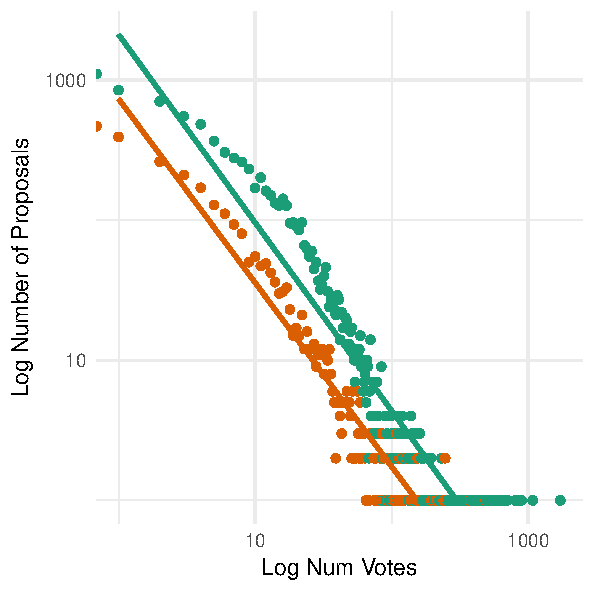
\includegraphics[width=1\textwidth]{Figures/votes_1.pdf}
        \caption{Probability Density Function}
    \end{subfigure}%
    ~ 
    \begin{subfigure}{0.5\textwidth}
        \centering        
        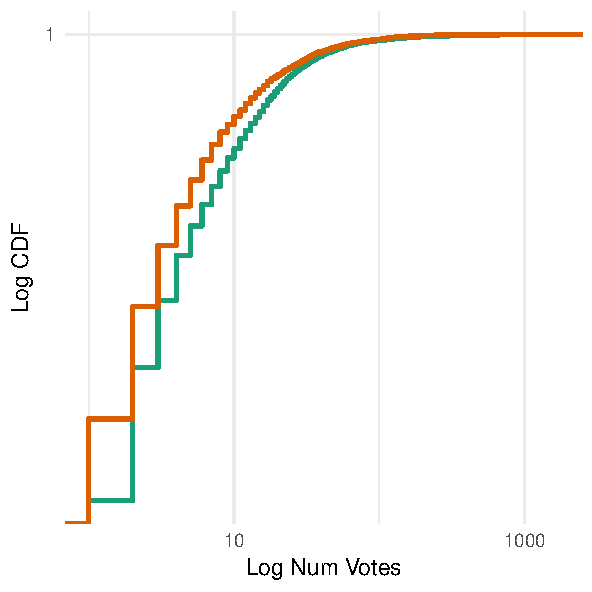
\includegraphics[width=1\textwidth]{Figures/votes_2.pdf}
        \caption{Cumulative Distribution Function}
    \end{subfigure}
    \caption{Number of votes on a proposal (green stands for the accepted ones and orange for the rejected): (a) on top of the density functions of votes we have fitted linearly each power law distribution. Both fits have the same slope, but the accepted proposals one is shifted to the right.}
    \label{votes}
\end{figure}

\subsection{Categorical features}\label{sec:catfeat}
The second subset of features to analyze refers to the categorical variables. These contain qualitative information, which ease the understanding of the proposals. These features are \emph{source} $s_i$, \emph{district} $d_i$, \emph{category} $k_i$, and \emph{subcategory} $sk_i$. 

The \emph{source} of the proposal $s_i$ determines which was the origin of the proposal. It takes four values: \emph{official} which corresponds to Barcelona's city council, \emph{citizen} corresponding to a single individual, \emph{organization} referring to an entity or group of people that represent a group of citizens, and finally the \emph{meeting} source, which corresponds to proposals originated \emph{in person} meetings organized by the city council. The proposals under this source are the the translation of the outcome of those reunions, where all citizens could attend and discuss some ideas.

If we observe the acceptance ratio  of a proposal based on the source (Figure \ref{source}), we clearly see how \emph{official} proposals originated by the city council have a high chance of being accepted compared with the other ones, e.g., citizen proposals. The platform initially contained more than $1,000$ petitions from the electoral program of the ruling party. This is highly influenced by the fact the initial proposals were built and thought following the strategic lines that the government would want to follow in the mandate. Therefore, they are proposals that the government already wanted to implement, and moreover, they where already viable proposals and within the scope of action of the city hall.

\begin{figure}[H]
    \centering
    \begin{subfigure}{0.5\textwidth}
        \centering
        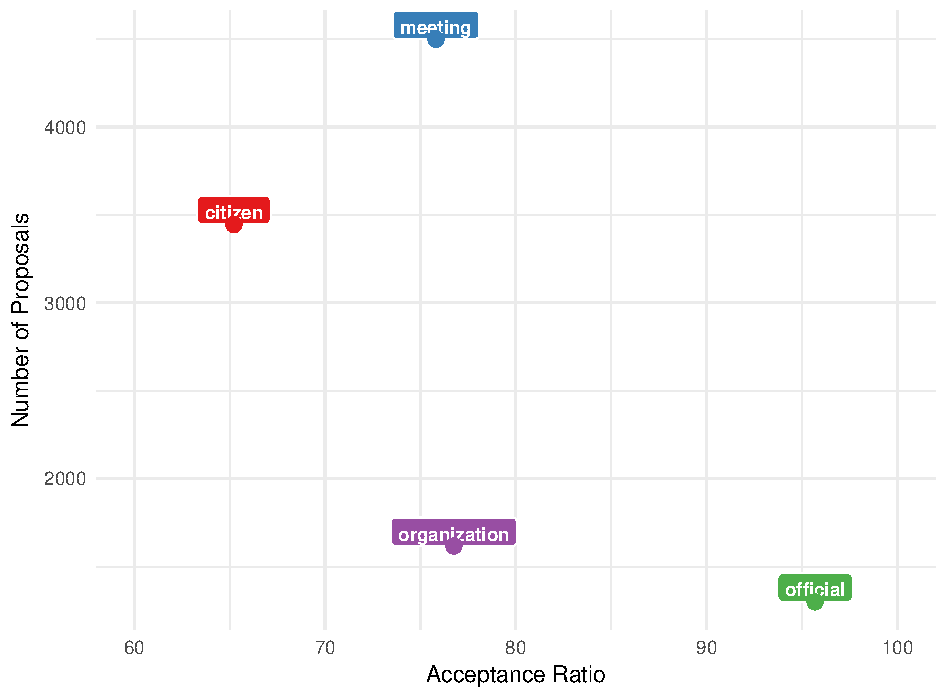
\includegraphics[width=\textwidth]{Figures/source_ac.pdf}
        \caption{}
    \end{subfigure}%
    ~ 
    \begin{subfigure}{0.5\textwidth}
        \centering        
        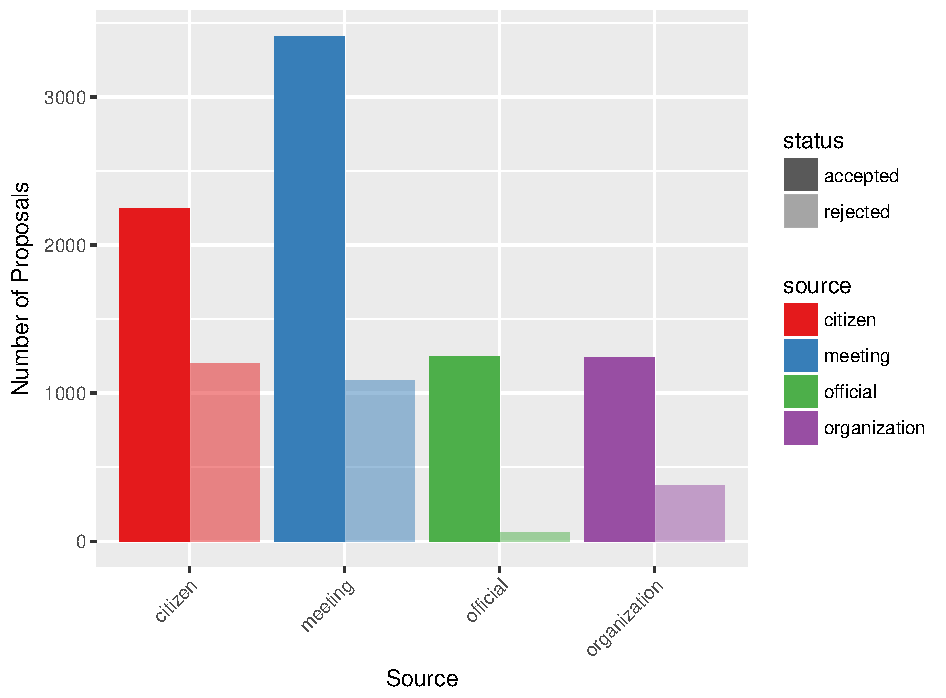
\includegraphics[width=\textwidth]{Figures/source_hist.pdf}
        \caption{}
    \end{subfigure}
    \caption{Accpetance / rejection of the proposals according to their origin. (a)~Relation between the acceptance ratio and the number of proposals for each different source.
(b) Absolute number of accepted/rejected proposals for each different source.}
    \label{source}
\end{figure}

Besides the \emph{source}, we have the \emph{district} $d_i$ category. Whitin this specific feature, proposals fall into two main categories, the ones where the scope is the whole city (are not bounded to an actual neighborhood) and the ones that are more tight to a specific local area. From what we know, the evaluation of the proposals was different depending on the scope. The ones related to just one district were evaluated by each district council independently of the category of the proposal while the ones where the scope was the city as a whole were split by each category and subcategory for evaluation. Due to this reason, we will analyze them separately. We will consider two types of models: a general one that comprises all the proposals and one for each specific district.

Figure \ref{district} shows the different acceptance rates per borough. We can see areas like \emph{Eixample}, \emph{Horta - Guinard\'o}, and \emph{Nou Barris} have really high acceptance ratios while proposals coming from \emph{Sarri\`a - Sant Gervasi} or \emph{Les Corts} are less likely to be accepted. As each district has its own administration, the differences we observe could be caused by a political misalignment and between governments with opposing  priorities. Those results diversity are also interesting for the prediction.

\begin{figure}[H]
\centering
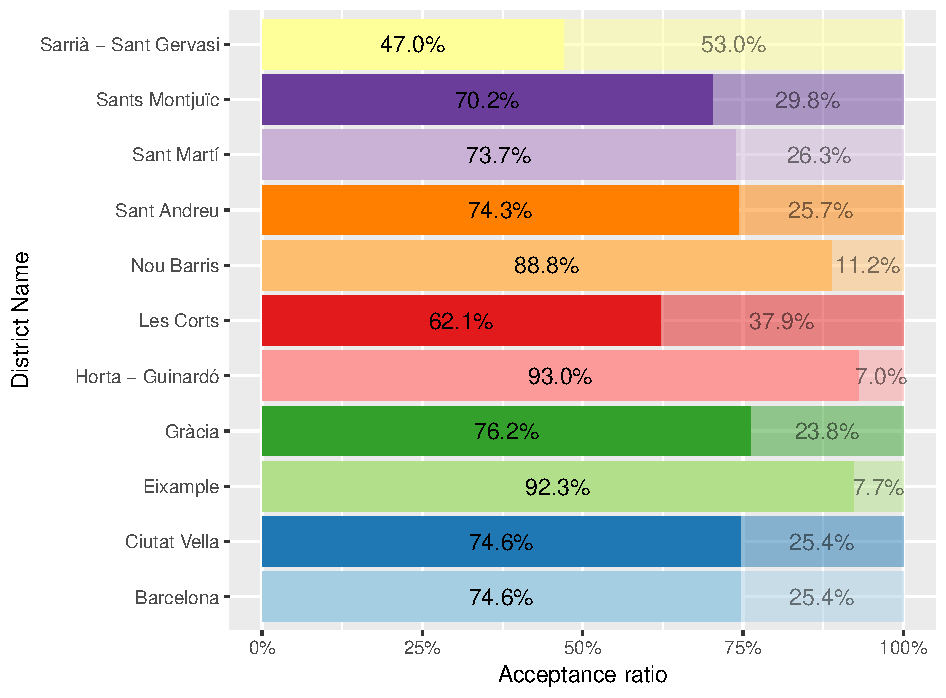
\includegraphics[width=\textwidth]{Figures/district.pdf}
\caption{Acceptance ratio per district}
\label{district}
\end{figure}

The last couple sets of features, \emph{category} $k_i$ and \emph{subcategory} $sk_i$, classify each proposal in its field of action, which are related to the five principal axis and multiple  strategic lines of actuation of the government. Those axis are \textit{Bon Viure}, which aims to improve quality of life, \textit{Transici\'o Ecol\`ogocia}, that tries to build a more sustainable city model, \textit{Economia Plural}, that takes care of the economical diversity, \textit{Bon Govern}, which commits to transparency and best governing practices, and \textit{Just\'icia Global}, which has an overall point of view and tries to fit within the international community. A more detailed overview can be found on the process' website \cite{pam}. 


Figure \ref{category} shows the acceptance of each of the main categories against the volume of proposals. Even the range of acceptance is quite small, ranging from 65\% in \textit{Just\'icia Global} to an almost 80\% in \textit{Economia Plural}. On the other hand, what we see as not being that balanced is the volume of proposals per category. This reflects both government and citizens priorities in a city in topics, being \textit{Bon Viure} the category with the biggest share of proposals, followed closely by \textit{Transici\'o Ecol\`ogocia}. Those two capture the proposals with a direct impact on the city and its inhabitants. The rest of the categories are less represented since the implications are not so clear on the peoples day to day life, making them less popular.

\begin{figure}[H]
    \centering
    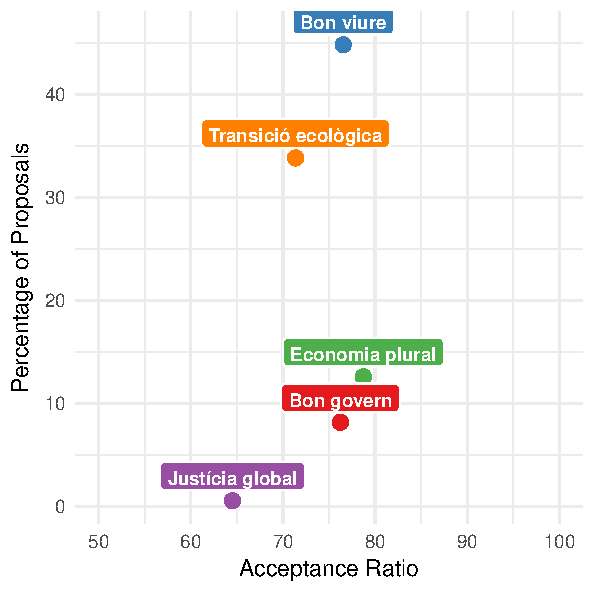
\includegraphics[width=0.66\textwidth]{Figures/category_1.pdf}
    \caption{Acceptance ratio per category}
    \label{category}
\end{figure}

Lastly, figure \ref{cat_dist} shows the acceptance ratios - which take a wider range of values (from 33\% to 100\%)-, are  not only by category but also per district, and illustrates how priorities differ significantly between neighborhoods. A clear example would be comparing \emph{Sants - Montjuic} and \emph{Sant Mart\'i} districts: on the first on,e the lowest acceptance ratio score is \textit{Transici\'o Ecol\`ogocia} with a 64,0\%, whereas on \emph{Sant Mart\'i} district is the category with the highest score, an 81,6\%. Now in \emph{Sant Mart\'i} we observe how \emph{Bon Govern} has the worst ratio (58,3\%) while on \emph{Sants - Montjuic} is one of the highest (82,0\%).

\begin{figure}[H]
    \centering
    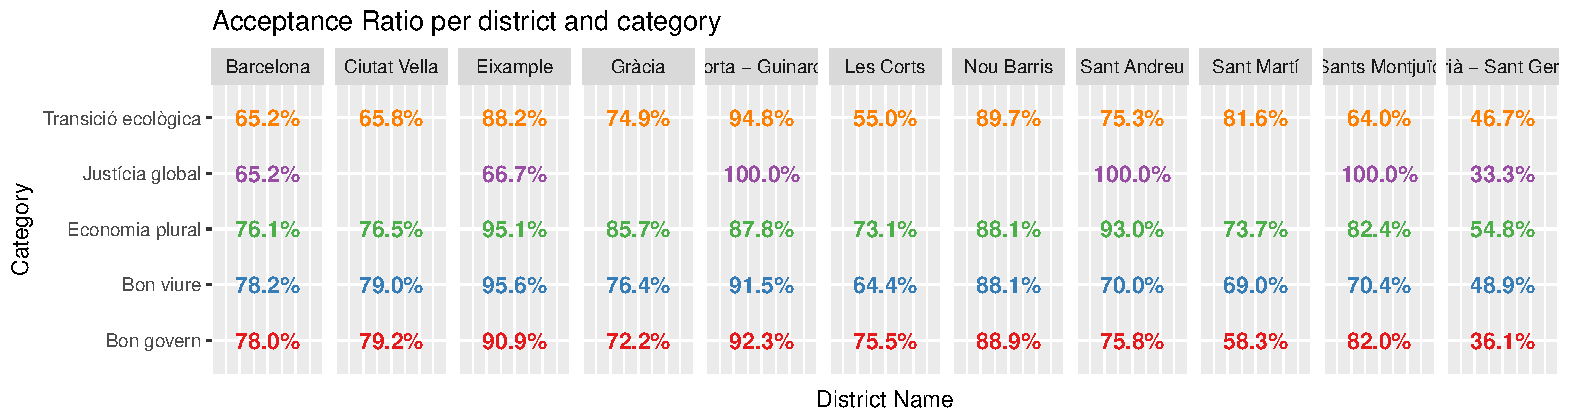
\includegraphics[width=\textwidth]{Figures/dist_cat.pdf}
    \caption{Acceptance ratio per category and district}
    \label{cat_dist}
\end{figure}

\section{Building a classifier}\label{sec:build}

After the previous global analysis, we introduce the methodology followed to estimate a statistical model. We have a very particular dataset where we find many typical 
complications that need to be adjusted for the implementation. 

To infer the acceptance or rejection of a proposal $i$, we have used a simple logistic regression model where the positive class ($y_i = +1$) represents the acceptance of the proposal and the negative class ($y_i=-1$) the rejection. The logistic regression model is widely used; it is the simplest model for classification, since feature values are combined linearly, it can be estimated efficiently and it provides some interpretability as done in similar problems \cite{navarro2017temporal}. 

Logistic regression, despite its name, is a linear model for classification rather than regression. Logistic regression is also known in the literature as \emph{logit regression}, \emph{maximum-entropy classification} or the \emph{log-linear classifier} \cite{logit}. In this model, the probabilities describing the possible outcomes of a single trial are modeled using the logistic function
\begin{equation}
P(y_i=+1) = \frac{1}{1+ \exp\left({-\beta_0-\sum^p_{j=1}\beta_jx_{i,j}}\right)},
\end{equation}
where the sum is over the $p$ feature values $x_{i,j}$ of proposal $i$, and $\beta~=~\{\beta_0,\beta_1,\hdots,\beta_p\}$ are the coefficients that needed to be estimated from the data. Notice that positive values of $\beta_l$ point out that $x_l$ has a positive effect on the acceptance of the proposal and, therefore, large values of that variable will make that event more likely.

To estimate the parameters $\beta$, we solve the following penalized least squares optimization problem:
%\begin{equation}
%\underset{w, c}{min\,} \frac{1}{2}w^T w + C \sum_{i=1}^n \log(\exp(- y_i (X_i^T w + c)) + 1) .
%\end{equation}
\begin{equation}
\underset{\beta, C}{\min\,} \left\{\frac{1}{2}\beta^T \beta + C \sum_{i=1}^n \log\left(1+ \exp\left({-\beta_0-\sum^p_{j=1}\beta_jx_{i,j}}\right)\right)\right\},
\end{equation}
where $C$ represents the inverse regularization strength, i.e., larger values of $C$ result in less regularization and vice-versa.

As the interpretability is one of the main purposes of using this algorithm, we also define a method to quantify how each feature contributes to the model. Importance is measured as the normalized percentage of the t-statistic for each model parameter. Logistic regression does not know how to deal with categorical features, therefore we must transforms each categorical feature with $m$ possible values into $m$ binary features, with only one active. This is known as one-hot encoding.

We will also compare the results obtained from the logistic regression against other classification algorithms to test if our results depend on the actual method implemented. The algorithm we will use specifically is Random Forests~\cite{rf}. Random forests are an ensemble learning method used in classification, that operate by constructing a multitude of decision trees at training time and outputting the class that is the mode of the classes. Random decision forests correct for decision trees' habit of overfitting to their training set. On figure \ref{random_forest} we show a schema of how the algorithm works, were each tree of the forest gives an output of the response variable and then the final class is defined by majority voting. unlike logistic regression, random forests are able to work with categorical variables, then we will not need to one-hot encode the variables.

\begin{figure}[h]
\centering
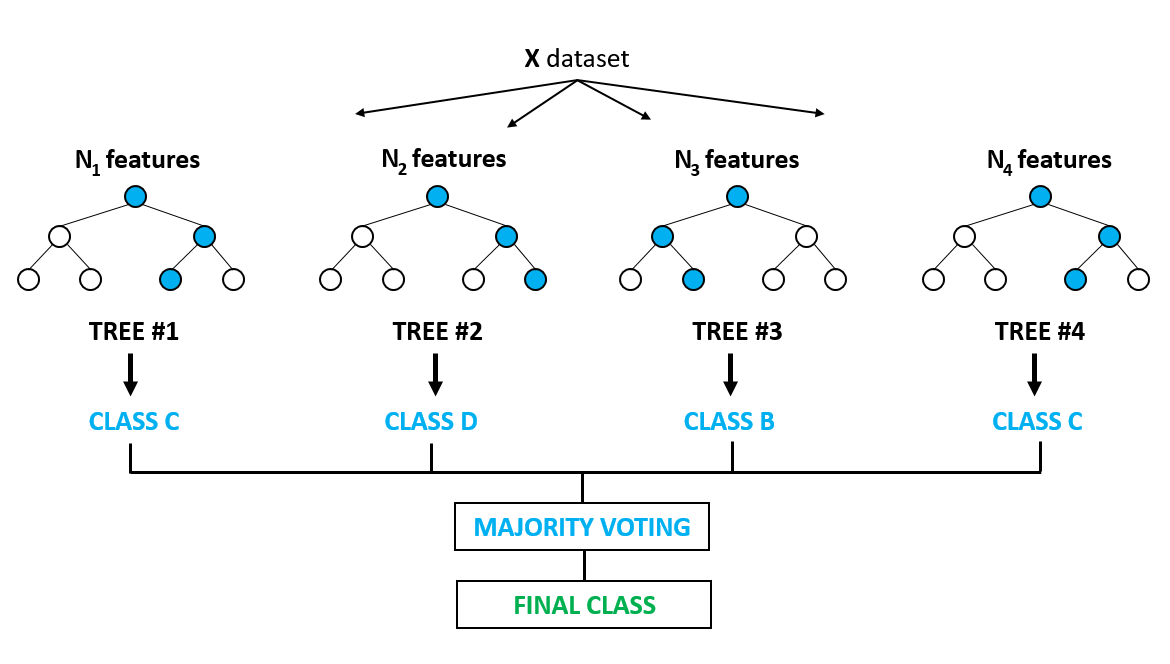
\includegraphics[width=\textwidth]{Figures/random_forests.png}
\caption{Random Forest Simplification}
\label{random_forest}
\end{figure}

After describing the model and objective, we now present some of the challenges that we need to address for this particular dataset of proposals.

\subsection{Skewed feature distributions}\label{sec:skewed}

The first problem we face is the distribution of our numeric features. In logistic regression classifiers, some kind of normalization is typically applied through transformations. This is specially important when variables have highly skewed distributions as we just seen before. In our case, all numeric features except $t_i$ are heavy-tailed distributed. Hence, we must log-transformed them before using them in our models.

Figure \ref{hists} shows the histograms of the feature values after transforming their values using the logarithm: the first row of charts corresponds to the comment related features (total, positive, neutral, and negative respectively) and the second row shows plots about the total number of users, number of votes, and days active in the platform.  We can see that the the distributions of the main variables used in our models are ``better behaved'' after the transformation.
Unlike before, the values are more concentrated and do not span more than two orders of magnitude.

\begin{figure}[h]
\centering
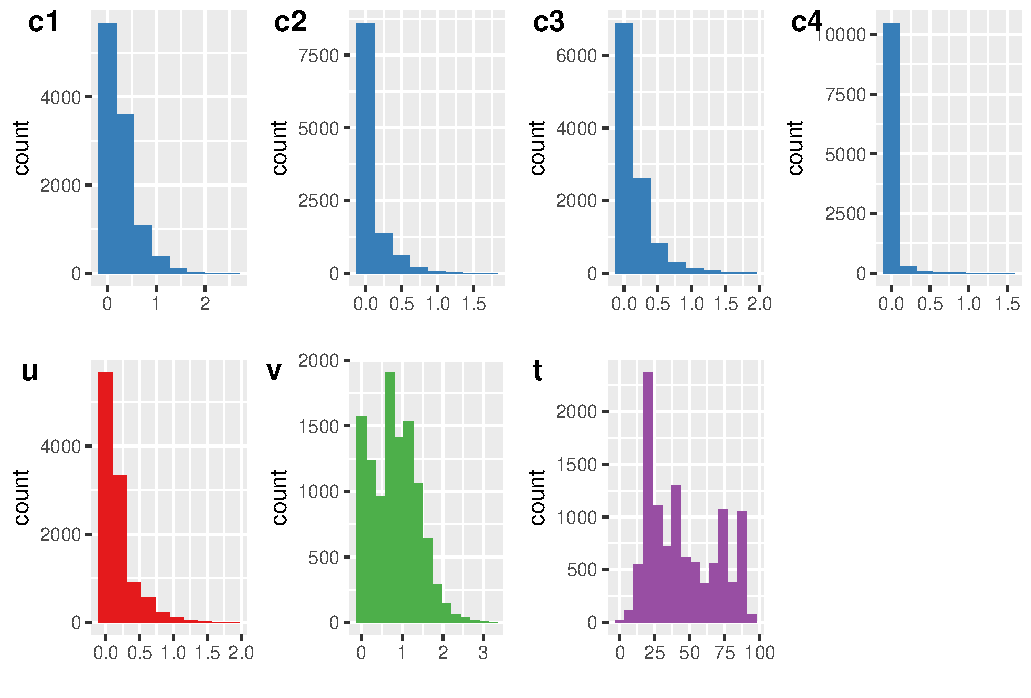
\includegraphics[width=\textwidth]{Figures/numerical_features.pdf}
\caption{Histograms of numerical log-transformed variables}
\label{hists}
\end{figure}

\subsection{Highly correlated features}\label{sec:corr}

The next problematic aspect that we have considered is the existence of highly correlated features. In these cases, one predictor variable may carry redundant information and the weight of this feature may be \emph{spread} among the other highly correlated features is that, even if all the variables are relevant to the predictive model. Correlated variables can diminish the predicting power and interpretability of a model and we need to understand the explanatory power between them before starting to construct a statistical significant model. The selection of features is addressed using the correlation matrix. As shown in Figure \ref{corr}, some of the variables have moderate correlation coefficients, which is expected since they all inform us of the activity in the platform.

The largest correlations are found between the total number of users $u_i$, the total number of comments $c_i$ and the total number of neutral comments. We choose to exclude $u_i$ and $c_i$ from the model. 

\begin{figure}[t!]
\centering
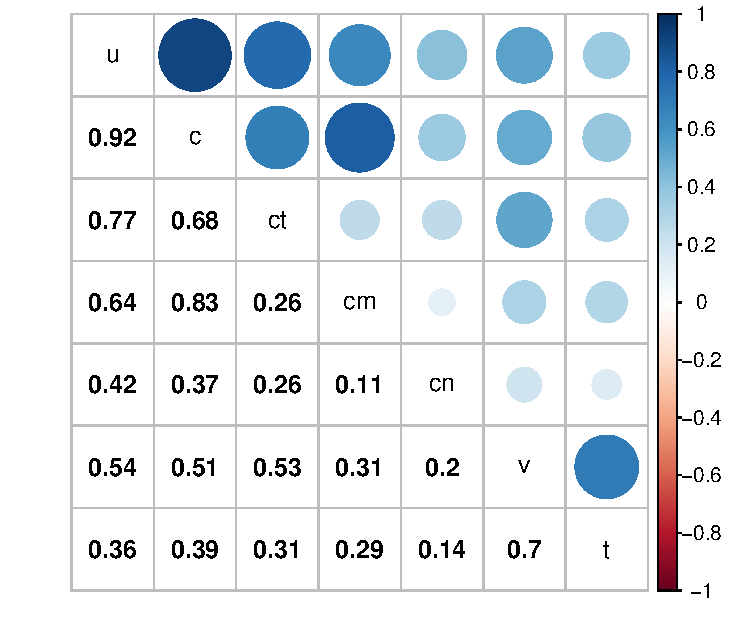
\includegraphics[width=0.75\textwidth]{Figures/corr.pdf}
\caption{Correlation matrix between features}
\label{corr}
\end{figure}

\subsection{Evaluation of the classifier - Unbalancedness}\label{sec:eval}

After these adjustments, we need to define a way to evaluate the model performance in a robust way in order to analyze its results, and, to do so we need to split our data into training and testing sets. One well-known widely-used method is $k-$fold cross-validation~\cite{cross-validation}.
In $k-$fold cross-validation, the whole dataset is randomly fractioned into $k$ equal sized subsamples. Of the $k$ partitions, a single one is retained as the test data for validating the model, and the remaining $k-1$ partitions are used as training data. The cross-validation process is then repeated $k$ times, with each of the partitions used exactly once as the test data. The results are then averaged to produce a single estimation. In our model, as in the majority of the literature, we used $k=10$.

The dataset that we are dealing with is unbalanced when it comes to the response variable, where 75\% of the proposals were accepted and only 25\% were rejected. This may cause problems when training the model so we need to do some sampling in order to equilibrate it. We have two options: we can either reduce the number of samples that represent the majority class or generate synthetic cases for the minority one. We compared both methods, using random under-sampling on one hand, and SMOTE~\cite{chawla2002smote} on the other and compared their performances. 

\begin{figure}[h]
    \centering
    \begin{subfigure}{0.5\textwidth}
        \centering
        \caption{No Re-sampling}
        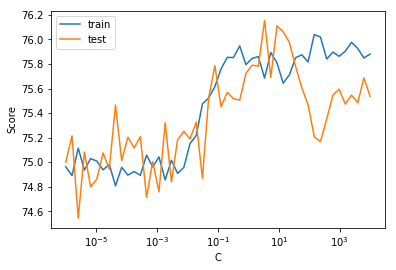
\includegraphics[width=1\textwidth]{Figures/no_resampling.png}
    \end{subfigure}%
    
    \begin{subfigure}{0.5\textwidth}
        \centering
        \caption{Random Under-sampling}
        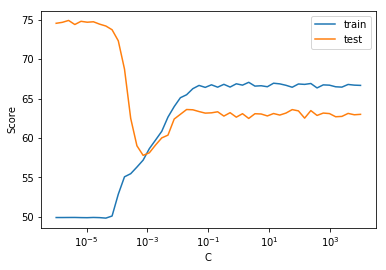
\includegraphics[width=1\textwidth]{Figures/undersampling.png}
    \end{subfigure}%
    ~ 
    \begin{subfigure}{0.5\textwidth}
        \centering
        \caption{Over-sampling with SMOTE}
        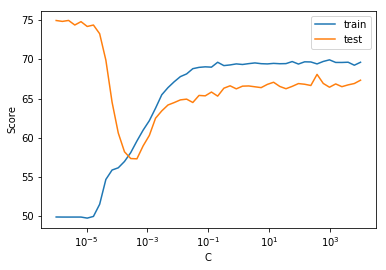
\includegraphics[width=1\textwidth]{Figures/oversampling.png}
    \end{subfigure}
    \caption{Comparison of the re-sampling techniques}
    \label{smote}
\end{figure}

On Figure \ref{smote} we observe a comparison between the two regularization methods mentioned earlier against not using any re-sampling technique. We plotted the train and test scores (where score is the accuracy of the logistic model fit) against the inverse of regularization strength $C$. On the left, the random under-sampling method achieves a $67\%$ accuracy on the train subset and $66\%$ on the test one. On the right, the SMOTE method shows a slightly better predicting potential, having a $69\%$ on train set and $67\%$ on test. Here the difference we observe is quite small, $\sim 2\%$, but for some models we want to build where the amount of data we dispose is not large, therefore we select SMOTE oversampling method as a solution to the unbalance of the data.

A common measure the performance of a model is the Area Under the ROC curve (AUC). The ROC curve~\cite{roc}, is a graphical plot which illustrates the performance of a binary classifier system as its discrimination threshold is varied. It is created by plotting the true positive rate vs. the false positive rate, at various threshold settings. TPR is also known as sensitivity, and FPR is one minus the specificity or true negative rate. ROC curves typically feature true positive rate on the Y axis, and false positive rate on the X axis. This means that the top left corner of the plot is the "ideal" point - a false positive rate of zero, and a true positive rate of one. This is not very realistic, but it does mean that a larger AUC is usually better. 

Being that said, ROC curves can present an optimistic view of the classifier performance if the distribution of the response variable is not well balanced, which is our case. For those kind of distributions, Precision-Recall curves \cite{prec_recall}. Precision-Recall is a useful measure of success of prediction when the classes are very imbalanced. In information retrieval, precision is a measure of result relevancy, while recall is a measure of how many truly relevant results are returned. A high area under the curve represents both high recall and high precision, where high precision relates to a low false positive rate, and high recall relates to a low false negative rate. They are therefore are an alternative to ROC because they evaluate the percentage of true positives among positive predictions.

To sum up, we will apply the over-sampling technique just on the train subset to not jeopardize the predictions with synthetic results and we will use the Area Under the Precision-Recall Curve (AUC) as a performance indicator metric. 

\newpage


